% ============================================================
%  Section 5 — Results
% ============================================================

\section{Results}
\label{sec:results}

\subsection{The price-age profile: Bordeaux vs.\ Burgundy}

Figure~\ref{fig:spline} plots the estimated natural cubic spline for all six groups against
normalised wine age. Panels~A and~B display the Bordeaux and Burgundy subgroups separately;
Panel~C juxtaposes the aggregate Bordeaux and Burgundy series. Through the pre-maturity period,
log prices rise monotonically for all groups — that much is uncontroversial. The divergence
comes after maturity.

Among Bordeaux wines, both the Grand Cru tier (1\textsuperscript{er} Cru Class\'es M\'edoc and
Premiers grands crus class\'es A, St\'emilion) and the Premier Cru tier (2\textsuperscript{nd}
through 5\textsuperscript{th} growths plus Graves and St\'emilion~B) exhibit a pronounced dip in
the trough zone ($a^* \in [1.6, 2.0)$, approximately 32--40 years of age). The Bordeaux Grand
Cru dip is the deepest, consistent with the longer maturity windows and higher consumption
valuations at peak for the most prestigious châteaux. Among Burgundy wines, Burgundy Grand Cru
continues to rise through the same window without interruption; Burgundy Premier Cru shows a
mild inflection but no sustained decline.

\begin{figure}[htbp]
  \centering
  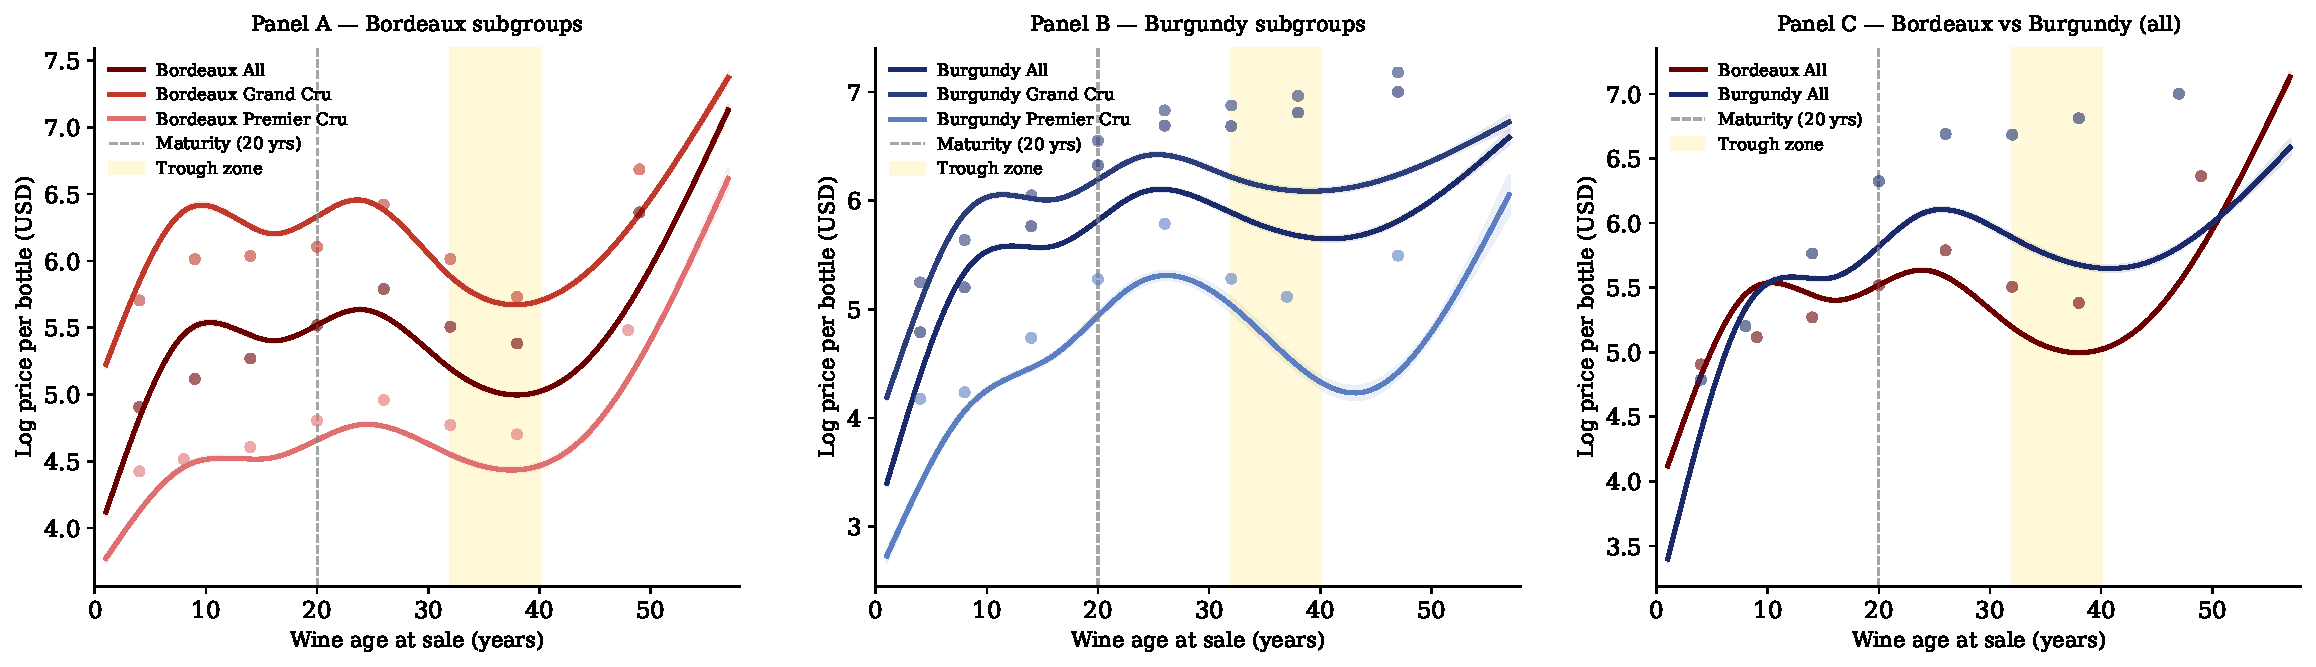
\includegraphics[width=\textwidth]{figures/fig_spline_comparison.pdf}
  \caption{Price-age profiles estimated by natural cubic spline (knots at
    $a^* \in \{0.4, 0.8, 1.2, 1.6, 2.2\}$) with 95\,\% confidence bands (shaded).
    \textit{Panel A}: Bordeaux subgroups (All, Grand Cru, Premier Cru).
    \textit{Panel B}: Burgundy subgroups (All, Grand Cru, Premier Cru).
    \textit{Panel C}: Bordeaux All vs.\ Burgundy All.
    Dots are binned medians (bin width: 0.30 normalised-age units).
    The dashed vertical line marks the maturity threshold (20 years);
    the shaded yellow band indicates the trough zone (approximately 32--40 years,
    $a^* \in [1.6, 2.0)$).
    $x$-axis is calendar age in years (normalised age $\times$ 20-year cap).
    Sample: 1996--2015 auction lots.}
  \label{fig:spline}
\end{figure}

\subsection{Statistical significance of the dip}

Tables~\ref{tab:segment_dip_bordeaux} and~\ref{tab:segment_dip_burgundy} report the segment
dummy regressions for Bordeaux and Burgundy groups respectively, each in four specifications:
(1) baseline, (2) vintage year fixed effects, (3) producer fixed effects, and (4) both fixed
effects simultaneously.

For Bordeaux Grand Cru, the trough segment is substantially below the peak segment across all
four specifications, and the Trough~$-$~Peak contrast is significant at the 0.1\,\% level.
Bordeaux Premier Cru likewise shows a statistically significant dip. The magnitudes are
broadly stable when adding vintage or producer fixed effects, confirming that the trough is not
a cohort quality effect or a producer compositional artifact.

Burgundy Grand Cru shows the opposite: the trough segment is \textit{above} the peak in all
specifications, consistent with a monotonically rising profile and the absence of
consumer-demand exit.

\begin{table}[htbp]
\centering
\caption{Price-age segment regression: Bordeaux groups}
\label{tab:segment_dip_bordeaux}
\resizebox{\textwidth}{!}{%
\begin{tabular}{lcccccccccccc}
\toprule
 & \multicolumn{4}{c}{Bordeaux All} & \multicolumn{4}{c}{Bordeaux Grand Cru} & \multicolumn{4}{c}{Bordeaux Premier Cru} \\
\cmidrule(lr){2-5}\cmidrule(lr){6-9}\cmidrule(lr){10-13}
Segment (base: young) & (1) & (2) & (3) & (4) & (1) & (2) & (3) & (4) & (1) & (2) & (3) & (4) \\
\midrule
\textit{Approach} & $0.179^{***}$ & $0.603^{***}$ & $0.179^{***}$ & $0.603^{***}$ & $0.058^{***}$ & $0.631^{***}$ & $0.058^{***}$ & $0.631^{***}$ & $0.117^{***}$ & $0.330^{***}$ & $0.117^{***}$ & $0.330^{***}$ \\
  & (0.005) & (0.005) & (0.005) & (0.005) & (0.006) & (0.006) & (0.006) & (0.006) & (0.005) & (0.005) & (0.005) & (0.005) \\
\textit{Peak} & $0.467^{***}$ & $1.385^{***}$ & $0.467^{***}$ & $1.385^{***}$ & $0.276^{***}$ & $1.433^{***}$ & $0.276^{***}$ & $1.433^{***}$ & $0.371^{***}$ & $0.860^{***}$ & $0.371^{***}$ & $0.860^{***}$ \\
  & (0.005) & (0.007) & (0.005) & (0.007) & (0.006) & (0.008) & (0.006) & (0.008) & (0.006) & (0.008) & (0.006) & (0.008) \\
\textit{Trough} & $0.163^{***}$ & $1.903^{***}$ & $0.163^{***}$ & $1.903^{***}$ & $-0.214^{***}$ & $1.977^{***}$ & $-0.214^{***}$ & $1.977^{***}$ & $0.228^{***}$ & $1.211^{***}$ & $0.228^{***}$ & $1.211^{***}$ \\
  & (0.008) & (0.012) & (0.008) & (0.012) & (0.010) & (0.013) & (0.010) & (0.013) & (0.011) & (0.014) & (0.011) & (0.014) \\
\textit{Antique} & $1.076^{***}$ & $2.597^{***}$ & $1.076^{***}$ & $2.597^{***}$ & $0.602^{***}$ & $2.735^{***}$ & $0.602^{***}$ & $2.735^{***}$ & $0.994^{***}$ & $1.673^{***}$ & $0.994^{***}$ & $1.673^{***}$ \\
  & (0.008) & (0.016) & (0.008) & (0.016) & (0.009) & (0.018) & (0.009) & (0.018) & (0.013) & (0.021) & (0.013) & (0.021) \\
\midrule
\textbf{Trough $-$ Peak} & $-0.304^{***}$ & $0.518$ & $-0.304^{***}$ & $0.518$ & $-0.490^{***}$ & $0.544$ & $-0.490^{***}$ & $0.544$ & $-0.143^{***}$ & $0.351$ & $-0.143^{***}$ & $0.351$ \\
  & (-26.2\%) & (+67.9\%) & (-26.2\%) & (+67.9\%) & (-38.8\%) & (+72.2\%) & (-38.8\%) & (+72.2\%) & (-13.3\%) & (+42.1\%) & (-13.3\%) & (+42.1\%) \\
\midrule
$R^2$ & 0.054 & 0.205 & 0.054 & 0.205 & 0.036 & 0.364 & 0.036 & 0.364 & 0.055 & 0.228 & 0.055 & 0.228 \\
$N$ & 436,413 & 436,413 & 436,413 & 436,413 & 215,036 & 215,036 & 215,036 & 215,036 & 221,377 & 221,377 & 221,377 & 221,377 \\
Vintage FE & No & Yes & No & Yes & No & Yes & No & Yes & No & Yes & No & Yes \\
Producer FE & No & No & Yes & Yes & No & No & Yes & Yes & No & No & Yes & Yes \\
\bottomrule
\end{tabular}
}
\par\vspace{4pt}
{\footnotesize\textit{Notes:} OLS, dependent variable log price per bottle (USD). Robust (HC1) standard errors in parentheses. Segments: \textit{young} = $a^* \in [0, 0.6)$; \textit{approach} $\in [0.6, 1.0)$; \textit{peak} $\in [1.0, 1.6)$; \textit{trough} $\in [1.6, 2.0)$; \textit{antique} $\in [2.0, 3.0]$. ``Trough $-$ Peak'' reports the direct contrast with one-sided $p$-value (trough $<$ peak). (1) Baseline. (2) Vintage FE. (3) Producer FE. (4) Both FE. $^{***}p<0.001$, $^{**}p<0.01$, $^{*}p<0.05$.}
\end{table}


\begin{table}[htbp]
\centering
\caption{Price-age segment regression: Burgundy groups}
\label{tab:segment_dip_burgundy}
\resizebox{\textwidth}{!}{%
\begin{tabular}{lcccccccccccc}
\toprule
 & \multicolumn{4}{c}{Burgundy All} & \multicolumn{4}{c}{Burgundy Grand Cru} & \multicolumn{4}{c}{Burgundy Premier Cru} \\
\cmidrule(lr){2-5}\cmidrule(lr){6-9}\cmidrule(lr){10-13}
Segment (base: young) & (1) & (2) & (3) & (4) & (1) & (2) & (3) & (4) & (1) & (2) & (3) & (4) \\
\midrule
\textit{Approach} & $0.625^{***}$ & $0.964^{***}$ & $0.625^{***}$ & $0.964^{***}$ & $0.477^{***}$ & $0.832^{***}$ & $0.477^{***}$ & $0.832^{***}$ & $0.621^{***}$ & $0.922^{***}$ & $0.621^{***}$ & $0.922^{***}$ \\
  & (0.006) & (0.006) & (0.006) & (0.006) & (0.007) & (0.007) & (0.007) & (0.007) & (0.010) & (0.010) & (0.010) & (0.010) \\
\textit{Peak} & $1.314^{***}$ & $1.951^{***}$ & $1.314^{***}$ & $1.951^{***}$ & $1.046^{***}$ & $1.699^{***}$ & $1.046^{***}$ & $1.699^{***}$ & $1.407^{***}$ & $2.174^{***}$ & $1.407^{***}$ & $2.174^{***}$ \\
  & (0.008) & (0.012) & (0.008) & (0.012) & (0.009) & (0.012) & (0.009) & (0.012) & (0.019) & (0.024) & (0.019) & (0.024) \\
\textit{Trough} & $1.505^{***}$ & $2.773^{***}$ & $1.505^{***}$ & $2.773^{***}$ & $1.271^{***}$ & $2.567^{***}$ & $1.271^{***}$ & $2.567^{***}$ & $1.154^{***}$ & $2.911^{***}$ & $1.154^{***}$ & $2.911^{***}$ \\
  & (0.017) & (0.029) & (0.017) & (0.029) & (0.018) & (0.029) & (0.018) & (0.029) & (0.045) & (0.075) & (0.045) & (0.075) \\
\textit{Antique} & $1.726^{***}$ & $3.438^{***}$ & $1.726^{***}$ & $3.438^{***}$ & $1.451^{***}$ & $3.215^{***}$ & $1.451^{***}$ & $3.215^{***}$ & $1.201^{***}$ & $3.654^{***}$ & $1.201^{***}$ & $3.654^{***}$ \\
  & (0.013) & (0.038) & (0.013) & (0.038) & (0.013) & (0.038) & (0.013) & (0.038) & (0.030) & (0.092) & (0.030) & (0.092) \\
\midrule
\textbf{Trough $-$ Peak} & $0.191$ & $0.821$ & $0.191$ & $0.821$ & $0.225$ & $0.869$ & $0.225$ & $0.869$ & $-0.253^{***}$ & $0.737$ & $-0.253^{***}$ & $0.737$ \\
  & (+21.0\%) & (+127.4\%) & (+21.0\%) & (+127.4\%) & (+25.3\%) & (+138.3\%) & (+25.3\%) & (+138.3\%) & (-22.4\%) & (+109.0\%) & (-22.4\%) & (+109.0\%) \\
\midrule
$R^2$ & 0.142 & 0.205 & 0.142 & 0.205 & 0.118 & 0.195 & 0.118 & 0.195 & 0.150 & 0.239 & 0.150 & 0.239 \\
$N$ & 308,648 & 308,648 & 308,648 & 308,648 & 221,512 & 221,512 & 221,512 & 221,512 & 87,136 & 87,136 & 87,136 & 87,136 \\
Vintage FE & No & Yes & No & Yes & No & Yes & No & Yes & No & Yes & No & Yes \\
Producer FE & No & No & Yes & Yes & No & No & Yes & Yes & No & No & Yes & Yes \\
\bottomrule
\end{tabular}
}
\par\vspace{4pt}
{\footnotesize\textit{Notes:} OLS, dependent variable log price per bottle (USD). Robust (HC1) standard errors in parentheses. Segments: \textit{young} = $a^* \in [0, 0.6)$; \textit{approach} $\in [0.6, 1.0)$; \textit{peak} $\in [1.0, 1.6)$; \textit{trough} $\in [1.6, 2.0)$; \textit{antique} $\in [2.0, 3.0]$. ``Trough $-$ Peak'' reports the direct contrast with one-sided $p$-value (trough $<$ peak). (1) Baseline. (2) Vintage FE. (3) Producer FE. (4) Both FE. $^{***}p<0.001$, $^{**}p<0.01$, $^{*}p<0.05$.}
\end{table}


\subsection{Piecewise linear robustness: negative trough slopes}

Table~\ref{tab:piecewise_slopes} reports the piecewise linear specification~\eqref{eq:piecewise}.
The trough slope $\beta_1 + \beta_2$ is negative for both Bordeaux groups (Bordeaux All:
$-0.020$; Bordeaux Grand Cru: $-0.261$), confirming that prices \emph{fall} with age in the
post-maturity period for Bordeaux wines. The deeper slope for Bordeaux Grand Cru reflects the
higher consumption valuations at peak maturity for the premier châteaux, which create a larger
correction when consumption buyers exit.

In contrast, the trough slope is positive and large for both Burgundy groups (Burgundy Grand
Cru: $+0.569$; Burgundy Premier Cru: $+0.403$), indicating that prices continue to rise
monotonically after maturity.

\begin{table}[htbp]
\centering
\caption{Piecewise linear price-age slopes by wine group}
\label{tab:piecewise_slopes}
\small
\begin{threeparttable}
\begin{tabular}{lcccccc}
\toprule
 & \multicolumn{1}{c}{Bx All} & \multicolumn{1}{c}{Bx GC} & \multicolumn{1}{c}{Bx PC} & \multicolumn{1}{c}{Bu All} & \multicolumn{1}{c}{Bu GC} & \multicolumn{1}{c}{Bu PC} \\
\midrule
$\beta_1$ (pre-maturity slope) & $0.6286^{***}$ & $0.4226^{***}$ & $0.4321^{***}$ & $1.6722^{***}$ & $1.3449^{***}$ & $1.5511^{***}$ \\
  & (0.0077) & (0.0101) & (0.0084) & (0.0099) & (0.0111) & (0.0172) \\
$\beta_2$ (change at maturity) & $-0.6487^{***}$ & $-0.6831^{***}$ & $-0.3265^{***}$ & $-1.0577^{***}$ & $-0.7757^{***}$ & $-1.1479^{***}$ \\
  & (0.0141) & (0.0175) & (0.0174) & (0.0226) & (0.0238) & (0.0498) \\
$\beta_3$ (change at antique) & $1.7404^{***}$ & $1.7145^{***}$ & $1.5738^{***}$ & $-0.5092^{***}$ & $-0.5041^{***}$ & $-0.5567^{***}$ \\
  & (0.0238) & (0.0266) & (0.0392) & (0.0449) & (0.0452) & (0.1257) \\
\midrule
\textbf{Trough slope} $\beta_1+\beta_2$ & $-0.0201^{**}$ & $-0.2606^{***}$ & $0.1056^{***}$ & $0.6145^{***}$ & $0.5692^{***}$ & $0.4032^{***}$ \\
  & (0.0086) & (0.0101) & (0.0116) & (0.0160) & (0.0163) & (0.0405) \\
\midrule
$R^2$ & 0.063 & 0.042 & 0.064 & 0.156 & 0.128 & 0.150 \\
$N$ & 436,413 & 215,036 & 221,377 & 308,648 & 221,512 & 87,136 \\
\bottomrule
\end{tabular}
\begin{tablenotes}
\footnotesize
\item Notes: OLS piecewise linear regression. Dependent variable: log price per bottle (USD).
  Model: $\log p = \alpha + \beta_1 a^* + \beta_2 (a^*-1)_+ + \beta_3 (a^*-2)_+ + \varepsilon$
  where $(x)_+ = \max(0,x)$.
  The slope in the trough zone ($a^* \in [1,2)$) is $\beta_1+\beta_2$; negative values indicate
  a declining price-age profile in the post-maturity period.
  Robust (HC1) standard errors in parentheses.
  $^{***}p<0.01$, $^{**}p<0.05$, $^{*}p<0.10$.
\end{tablenotes}
\end{threeparttable}
\end{table}


\subsection{Mechanism: collector composition and the price floor}

Table~\ref{tab:summary_stats} documents the key cross-sectional difference that rationalises
the contrasting profiles. Among young lots ($a^* < 0.4$, i.e., wines under 8 years old),
Burgundy Grand Cru commands the highest share of transactions above \$200 per bottle,
followed by Bordeaux Grand Cru and Bordeaux All, with Burgundy Premier Cru at the bottom.
The high entry price of Burgundy Grand Cru screens out consumption buyers from the outset:
a bidder who intends to drink the wine must be willing to pay collector-level prices even when
the wine is young. There is no consumption demand segment to exit at peak maturity, hence no
downward price pressure in the trough zone.

\begin{table}[htbp]
\centering
\caption{Sample summary statistics by wine group}
\label{tab:summary_stats}
\small
\begin{threeparttable}
\begin{tabular}{lrrrrrrr}
\toprule
 & & \multicolumn{2}{c}{Share} & \multicolumn{3}{c}{Median price (\$/bottle)} & \\
\cmidrule(lr){3-4}\cmidrule(lr){5-7}
Group & $N$ & Post-mat. & Coll.$^{a}$ & Young & At peak & Antique & Med. age \\
 & & (\%) & (\%) & & & & (yrs) \\
\midrule
Bordeaux All & 436,413 & 35.2 & 39.0 & \$140 & \$237 & \$532 & 16 \\
Bordeaux Grand Cru & 215,036 & 39.8 & 68.5 & \$336 & \$431 & \$748 & 17 \\
Bordeaux Premier Cru & 221,377 & 30.6 & 19.1 & \$85 & \$118 & \$220 & 14 \\
\midrule
Burgundy All & 308,648 & 18.5 & 36.8 & \$133 & \$504 & \$1,074 & 11 \\
Burgundy Grand Cru & 221,512 & 21.5 & 51.5 & \$213 & \$635 & \$1,278 & 11 \\
Burgundy Premier Cru & 87,136 & 10.9 & 11.2 & \$65 & \$170 & \$231 & 9 \\
\bottomrule
\end{tabular}
\begin{tablenotes}
\footnotesize
\item Notes: ``Young'' = age\textsubscript{norm} $<$ 0.4 ($<$ 8 years).
  ``At peak'' = age\textsubscript{norm} $\in$ [0.9, 1.1] (18--22 years).
  ``Antique'' = age\textsubscript{norm} $>$ 2.0 ($>$ 40 years).
  $^{a}$ Share of young lots priced $>$ \$200/bottle.
  Maturity cap: 20 years. Sample period: 1996--2015.
\end{tablenotes}
\end{threeparttable}
\end{table}


\subsection{Heterogeneity by wine-specific maturity}
\label{sec:results:heterogeneity}

\noindent\textit{[To be completed. Key result to document: the dip is not an artifact of
the maturity normalisation. Within the Bordeaux Grand Cru group, wines with shorter
maturity windows (say, $\tau_i < 18$ years) exhibit a shallower trough than wines with
longer maturity windows ($\tau_i \geq 22$ years), consistent with Proposition~\ref{prop:compstat}(iii)
--- a sharper consumption peak deepens the trough.
Show Table~X stratifying segment regression by tercile of $\tau_i$.]}

\subsection{Price-age medians: raw evidence}
\label{sec:results:medians}

Appendix~\ref{app:medians} reports binned log price medians by normalised age bin (width 0.2)
for all six groups. The raw medians confirm the spline shape without any smoothing assumption.
